%%%%%%%%%%%%%%%%%%%%%%%%%%%%%%%%%%%%%%%%%%%%%%%%%%%%%%%%
%%%%%%%%%%%%%%%%%%%%%%%%%%%%%%%%%%%%%%%%%%%%%%%%%%%%%%%%
\section{Materials and Methods}
%%%%%%%%%%%%%%%%%%%%%%%%%%%%%%%%%%%%%%%%%%%%%%%%%%%%%%%%
%%%%%%%%%%%%%%%%%%%%%%%%%%%%%%%%%%%%%%%%%%%%%%%%%%%%%%%%
%
FIM 3 is a fully operational pipeline of software tools to help acquire datasets, cache hydrofabrics, produce FIMs, and evaluate results.
%
%%%%%%%%%%%%%%%%%%%%%%%%%%%%%%%%%%%%%%%%%%%%%%%%%%%%%%%%
\subsection{Software Dependencies and Architecture}
%%%%%%%%%%%%%%%%%%%%%%%%%%%%%%%%%%%%%%%%%%%%%%%%%%%%%%%%
%
OWP FIM exclusively utilizes free and open source software dependencies including Python 3, GDAL, TauDEM, Geographic Resource Analysis Support System (GRASS), GNU Parallel, and MPICH \cite{python382,gdal2020,tarboton2005terrain,grass2020,tange2015gnu,amer2021mpich}.
Within the Python 3 ecosystem, many common packages are employed including but not limited to RichDEM, GeoPandas, Rasterio, Rasterstats, and Numba \cite{barnes2018richdem,jordahl2014geopandas,lam2015numba}. 
To simplify setup and enhance portability across host operating systems OWP FIM packages all dependencies up in Docker image (\url{https://docs.docker.com/engine/install/}). 
A user only need to install Docker on their host machine and build the image from the provided recipe. 

The FIM 3 pipeline is discretized into key areas that a user can interact with to reproduce the results of this study. Preprocessing acquires and prepares datasets for production of the FIM 3 hydrofabric. 
Producing the FIM hydrofabric produces the datasets required to make an inundation map including the relative elevation model (REM) or HAND grid, the catchments in vector and raster form, and the hydro-table (contains synthetic rating curves and cross-walk information).
%
%%%%%%%%%%%%%%%%%%%%%%%%%%%%%%%%%%%%%%%%%%%%%%%%%%%%%%%%
\subsection{Datasets}
\label{ssec:datasets}
%%%%%%%%%%%%%%%%%%%%%%%%%%%%%%%%%%%%%%%%%%%%%%%%%%%%%%%%
%
Most data sources used within FIM 3 are publicly available from a variety of government sources including the USGS, NWC, Federal Emergency Management Agency (FEMA), and US Army Core of Engineers (USACE) to enhance reproducibility and collaboration among government, academia, and industry.
The National Hydrography Dataset Plus High Resolution (NHDPlusHR) Beta Version is the latest hydrography dataset used for land surface hydrologic modeling in the US \cite{moore2019user}. 
It is used in conjunction with the hydrofabric of the NWM V2.1 to help define flowlines for FIM 3 while the NWM hydrofabric is also used to define reservoirs for exclusion and catchments to cross-walk to for forecasting purposes.
For enforcing levee data into the NED DEMs, the USACE National Levee Database (NLD) is used via burning feature elevations \cite{engineers2016national}.
Additionally, FEMA Base Level Engineering (BLE) from Region 6 (parts of Texas, Oklahoma, Arkansas, Louisiana and New Mexico) 1\% (100 year) and 0.2\% (500 year) datasets are used as validation in this study \cite{fema2021base,fema2021estimated}. 
These BLE datasets are provided at the watershed scale (HUC8) utilizing best available simulations and DEMs.
The full input datasets presented by source are list in Table \ref{tab:data}.
\note[Fernando Aristizabal]{Check Brian Avant, Trevor Grout, Bradford Bates, Ryan Spies}
%

\begin{table}
\caption{Data sources, names, and descriptions.}
\label{tab:data}
\centering
\begin{tabular}{|p{2cm}|p{4cm}|p{8cm}|}
%\begin{tabular}{l c c}
\hline
Source & Name & Description \\
\hline
USGS & NHDPlusHR BurnLineEvents & Stream lines used by NHDPlus HR for hydro-enforcement \\
\hline
USGS & NHDPlusHR Value-Added Attributes & Database of additional attributes associated with the BurnLineEvents that enhance navigation, analysis, and display \\
\hline
USGS & NHDPlusHR DEM & DEM used for NHDPlus HR at 1/3 arc-second (10m) spatial resolution and vertical units in centimeters \\
\hline
NOAA-OWP & NWM Streams & Stream network center lines used by NWM for routing and forecasting \\
\hline
NOAA-OWP & NWM Catchments & Surface drainage area corresponding to each reach in the NWM \\
\hline
NOAA-OWP & NWM Waterbodies & Waterbodies considered by the NWM as resevoirs or lakes \\
\hline
USACE & NLD & Levee database of locations and elevations  \\
\hline
WHERE? & Land-Sea Border & Border of land and sea and land and Great Lakes \\
\hline
FEMA & Cross-Sections & HEC-RAS cross-sections used for modeling in BLE datasets. Include discharges for 1\% and 0.2\% recurrence interval events \\
\hline
FEMA & Flood Inundation Extents & Extents produced by FEMA BLE for 1\% and 0.2\% recurrence interval events \\
\hline
\end{tabular}
\end{table}

Areas with all the required data (from the NWM and the USGS) are labeled as the FIM domain. 
\note[Fernando Aristizabal]{For Nick Chadwich} This includes XXXX HUC4's, XXX HUC'6s, and XX HUC8's.
An enhancement of OWP FIM v3 `Cahaba' over previous FIM versions is the support for Hawaii and Puerto Rico which the NWM v2.1 will cover.
%
%%%%%%%%%%%%%%%%%%%%%%%%%%%%%%%%%%%%%%%%%%%%%%%%%%%%%%%%
\subsection{Hydro-conditioning}
\label{ssec:hydro_conditioning}
%%%%%%%%%%%%%%%%%%%%%%%%%%%%%%%%%%%%%%%%%%%%%%%%%%%%%%%%
%
The DEM from the NED is subject to a series of hydro-conditioning procedures to enhance it's suitability for riverine flood inundation mapping. 
These techniques are specific for making OWP FIM and differ from the conditioning methods used by the NHDPlusHR Beta \cite{moore2019user}.
Hydro-conditioning is implemented to obtain many objectives including enforcing the location of hydrologically relevant features such as flowlines, lakes, or drainage divides whether natural or anthropogenic. 
It can also be used to simulate more accurate bathymetry which is not accounted for in the NED 10m DEM \cite{gesch2002national}.

Specifically within the context of FIM 3, the hydro-conditioning operations that take place in sequential order are presented. 
Prior to any hydro-conditioning, all input datasets must be subset from their original spatial domain scales into the processing unit designated at run time which can be either HUC 4, 6 or 8. 
The subsetting is done by spatial query for the cases of the levees, DEM, and NWM hydrofabric while the NHDPlusHR BurnLineEvents are subset via attribute query for the given reachcode's membership in the processing unit.
Hydro-conditioning raster operations take place on buffered boundary definitions to avoid edge contamination and effects \cite{lindsay2013measuring}. 
%
%%%%%%%%%%%%%%%%%%%%%%%%%%%%%%%%%%%%%%%%%%%%%%%%%%%%%%%%
\subsubsection{Stream Network Enforcement} 
\label{ssec:stream_network_enforcment}
%
\note[Fernando Aristizabal]{For Brian Avant}
The location of the stream network are enforced to ensure general agreement with established stream networks.
The NHDPlus HR Beta Burnline Event layer is used to enforce stream locations in the NHDPlusHR workflow so it is also used here for hydro-enforcement \cite{moore2019user}. 
However, to better match the drainage density of the NWM V2.1 stream network which is based on the NHDPlus Medium Resolution, the Burnline Events are pruned utilizing a nearest neighbor search around the NWM flowlines. 
Pruning the NHD network is completed at for every NWM V2.1 headwater point where the nearest NHDPlusHR Burline Event feature is selected and downstream features are also selected.
The resulting pruned NHD stream network is what gets hydro-enforced in subsequent operations.
This procedure is best illustrated in Figure \ref{fig:stream_density_pruning} which shows that the pruned NHD network corresponds to the full density NHD network at NWM V2.1 headwater locations only. 
Additionally, the NHDPlusHR pruned headwaters are later used for seeding a new FIM drainage network that best agrees with the DEM after all hydro-conditioning takes place.
%
\begin{figure}[h!]
\centering
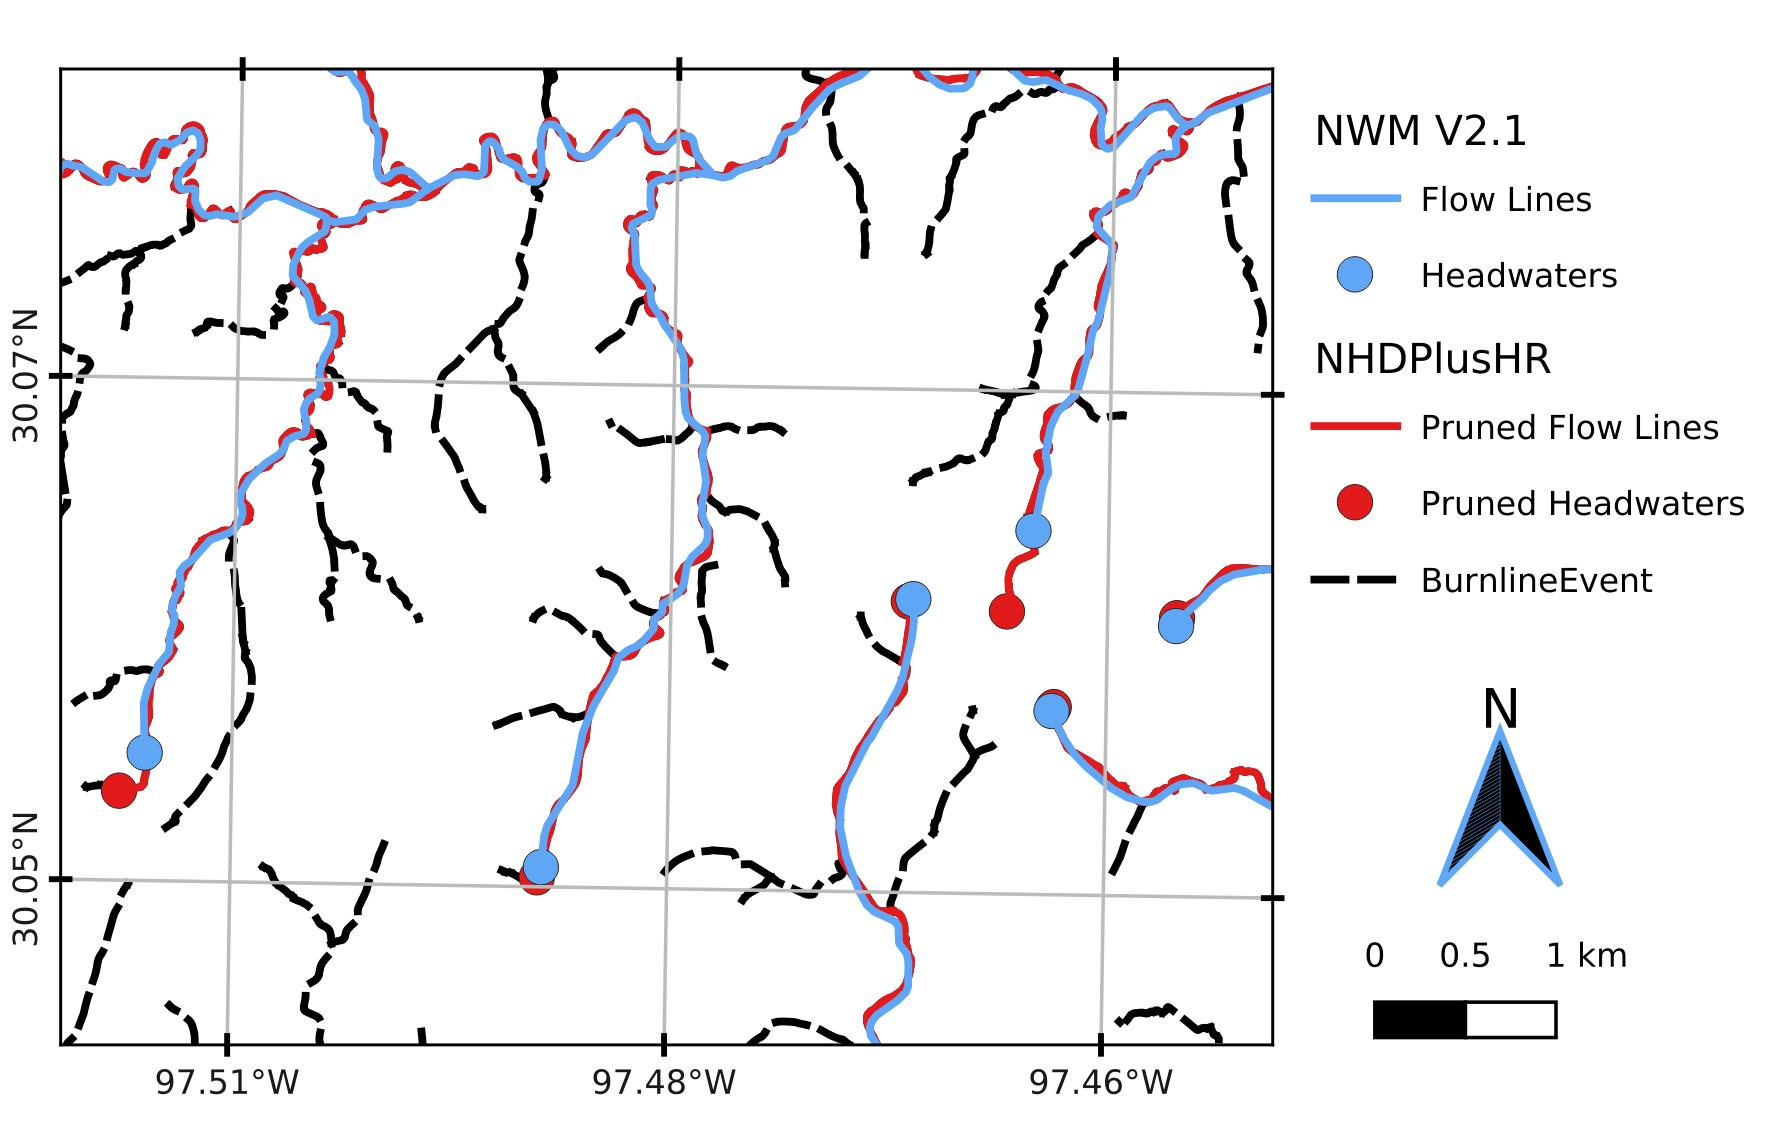
\includegraphics[scale=1.0]{figures/headwaters.jpg}
\caption{Pruning of NHDPlus HR Beta Burnline Events (dotted black) to NWM V2.1 stream density (blue) using nearest neighbor selection. Resulting stream network (red) matches the drainage density of NWM V2.1 while corresponding spatially with the NHDPlusHR Burnline Events.}
\label{fig:stream_density_pruning}
\end{figure}
%
This results in a stream network that has the same density as the NWM V2.1 flowline network but utilizes the locations of the NHDPlusHR Beta BurnLineEvents. 

\note[Fernando Aristizabal]{For Trevor Grout}
The pruned stream network is then utilized to hydro-enforce the DEM with a methodology developed by \citeA{hellweger1997agree} known as the AGREE DEM Surface Reconditioning System. 
The AGREE algorithm seeks to burn artificially deep thalweg elevations by a uniform value known as sharp drop. 
The modification continues by excavating an area of a given buffer distance from the thalweg by a depth proportional to the distance from the channel given by the smooth drop. 
The resulting enforcement of the thalweg and general bathymetric region results in a cross-section resembling a trapezoidal shape with a significantly lower elevation along the thalweg line only.
In total, the AGREE algorithm requires three parameters including the buffer distance, smooth drop, and sharp drop. 
Using simple thalweg burning techniques as opposed to the full AGREE method helps prevent distortions in the delineation of streams as well as the catchment boundaries \cite{saunders1995grid,saunders1996gis,mizgalewicz1996modeling,hellweger1997agree,quenzer1998gis,baker2006comparison}.
\citeA{baker2006comparison} noted AGREE produced satisfactory results when compared to other enforcement especially when computational costs are considered. 
Downsides to the technique include the possibility of exhibiting parallel streams where the burned stream and real stream are both represented \cite{hellweger1997agree,saunders1999preparation} and some distortion of the catchment boundaries can also be observed \cite{saunders1999preparation,saunders1996gis}. Some of these drawbacks are later addressed by additional conditioning techniques later on.
%
%%%%%%%%%%%%%%%%%%%%%%%%%%%%%%%%%%%%%%%%%%%%%%%%%%%%%%%%
\subsubsection{Levee Enforcement}
%
\note[Fernando Aristizabal]{For Ryan Spies}
The National Elevation Dataset at 10m resolution lacks sufficient representation of fine grain features such as levees and embankments.
In order to better represent the influences of these features upon hydraulics and inundation extents, the National Levee Database (NLD) published by USACE was used to enforce elevations within the 10m DEM.
%
%%%%%%%%%%%%%%%%%%%%%%%%%%%%%%%%%%%%%%%%%%%%%%%%%%%%%%%%
\subsubsection{Depression Filling}
\label{sssec:depression_filling}
%
Local depressions are naturally occurring features of a DEM but must be addressed if a connected drainage network with continuous catchments are to be derived for flood modeling purposes.
The conditioned DEM was removed of depressions by filling areas with pits while preserving the stream and levee information previously enforced.
Priority-Flood developed by \citeA{barnes2014priority} is an algorithm for filling said depressions and shown to have improved performance over early works in the field by \citeA{jenson1988extracting} implemented in \citeA{tarboton2005terrain} as well as \citeA{planchon2002fast}.
The depression filling algorithm used in our pipeline is a Priority-Flood variant developed by \cite{zhou2016efficient} with enhanced single-thread performance and a time complexity of O(n log n) for floating point grids.
This performance was enabled by limiting the processing queue with a region-growing method to exclude many of the slope cells \cite{zhou2016efficient}.
The depression technique employed here does leave the existence of flat regions where pits existed aprior thus later requiring the need for resolving these flats.
The enhanced variant of Priority-Flood is implemented and made available by \citeA{barnes2018richdem} and \citeA{zhou2015filldem}.
%
%%%%%%%%%%%%%%%%%%%%%%%%%%%%%%%%%%%%%%%%%%%%%%%%%%%%%%%%
\subsubsection{Stream Thalweg Elevation Conditioning}
\label{sssec:stream_thalweg_elevation_conditioning}
%
Thalweg elevations are critical components of relative elevation based inundation mapping thus much is performed to ensure the best available, monotonically decreasing elevations are derived prior to normalizing of elevations.
In order to prevent situations where the burned thalweg and the thalweg endemic to DEM run parallel to one another, the normalized excavation algorithm \cite{saunders1999preparation} is used to seek a zonal (nearest neighbor) elevation minimum for each thalweg pixel. 
Each zone is defined as the thalweg's pixel nearest neighborhood within a maximum distance of 50m.
The zonal minimum is computed for each thalweg pixel zone and the minimum is used to replace the existing thalweg elevation value.

The next step involves conditioning these local minimums along the thalweg to enforce monotonically decreasing thalweg elevations for FIM.
\citeA{garousi2019terrain} proposed an algorithm that traverses stream thalweg pixels in a depth first manner starting with adding all the headwater pixels to a queue. 
The connectivity of the thalweg pixels is defined by the D-8 flow directions further discussed in Section \ref{ssec:flow_direction_and_flat_resolution}.
At every thalweg pixel, the minimum elevation among itself and its upstream contributing thalweg pixels is taken as shown in equation \ref{eq:thalweg_breach},
%
\begin{equation}
\label{eq:thalweg_breach}
\textbf{D}[x] = \min_{y\ drains\ to\ x} {(\ \textbf{D}[x]\ ,\ \textbf{D}[y]\ )}
\end{equation}
%
, in which \textbf{D} represents the array of thalweg adjusted elevations indexed by x and y where by y is upstream of x. 
When a pixel's upstream neighbors are all evaluated, the downstream pixel is added into the queue thus the depth first traversal of the drainage network.
This procedure enforces the location of streams and ensures that thalweg elevations are hydrologically correct which yielded a 7\% improvement in critical success index (CSI) per an evaluation for an event in 2017 on the Malad river \cite{garousi2019terrain}.
%
%%%%%%%%%%%%%%%%%%%%%%%%%%%%%%%%%%%%%%%%%%%%%%%%%%%%%%%%
\subsection{Deriving FIM Hydrofabric}
\label{ssec:deriving_fim_hydrofabric}
%%%%%%%%%%%%%%%%%%%%%%%%%%%%%%%%%%%%%%%%%%%%%%%%%%%%%%%%
%
The FIM Hydrofabric is defined here as the collection of geospatial datasets that are used for converting NWM discharges into inundation extents.
%
%%%%%%%%%%%%%%%%%%%%%%%%%%%%%%%%%%%%%%%%%%%%%%%%%%%%%%%%
\subsubsection{Flow Directions and Flats Resolution}
\label{ssec:flow_direction_and_flat_resolution}
%
To facilitate the generation of a connected stream network and its associated catchments from the conditioned DEM, the depression-filled DEM is used to derive connectivity in the form of D-8 flow directions.
D-8 seeks to allocate a drainage direction for every pixel based on the adjacent eight pixel neighborhood with the steepest slope \cite{o1984extraction}.
The horizontal component of slope is defined as one for the 4 neighboring pixels in the main cardinal directions while the intercardinal pixels are designated a horizontal component of $\sqrt{2}$. 
The flow direction is encoded as integers 1 through 8 corresponding with the cardinal direction East as 1 and continuing counter-clockwise to the Southwest direction as 8. 
Flow directions are derived for non-depression filled regions trivially with the above procedure but to define connectivity for every grid cell the remaining flats corresponding to depression filled cells must be resolved.

Flat resolution from flats endemic to the DEM or from depression filled regions is a costly,non-trivial procedure which was originally addressed by \citeA{garbrecht1997assignment}.  
Software implementations have developed means to partition the problem and resolve flats iteratively with communication across processes \cite{tarboton2009generalized,tesfa2011extraction,wallis2009parallel,tarboton2005terrain}.
The excessive iteration and communication leads to poor computational performance which motivated further work on how to optimize flat resolution \cite{survila2016scalable,barnes2014efficient}.
Specifically the work by \citeA{survila2016scalable} enables the use of parallel processing and made smoother catchments from our informal experience than those from \citeA{barnes2014efficient}.
By processing flats local to each partition separately from flats shared with other partitions, the accelerated flat resolution algorithm demonstrated an average speed up of 468x when compared to prior implementations \cite{survila2016scalable}.
OWP FIM 3 utilized a CyberGIS implementation of the D-8 flow direction algorithm with the accelerated resolution of flats \cite{survila2016scalable,cybergis2016}.
%
%%%%%%%%%%%%%%%%%%%%%%%%%%%%%%%%%%%%%%%%%%%%%%%%%%%%%%%%
\subsubsection{Deriving FIM Stream Network}
\label{sssec:deriving_fim_stream_network}
%
\note[Fernando Aristizabal]{For Brian Avant}
The derivations of relative elevations and catchments from the newly conditioned DEM involves re-deriving a new FIM stream network. 
The FIM stream network is of the same density as the NWM V2.1 network and fully converges at all junctions leaving no divergences in the network.
This is accomplished by using the seed points generated from the stream network enforcement process (Section \ref{ssec:stream_network_enforcment}).
These seeds points are headwater locations of the NHDPlusHR Beta Burnline Events layer that spatially correspond to the headwater definitions in the stream network of the NWM V2.1.
Feeding the seed points and previously computed flow directions into flow accumulation methods \cite{wallis2009parallel,tarboton1997new,tarboton2005terrain} yields a stream link accumulation raster that can be converted to a vector file for further processing.
Each stream link in this derived FIM stream network is split into equidistant reaches.
Stream links are defined here as segments of rivers discretized by junctions with other NWM river segments.
Stream links are then further segmented at NWM lakes and HUC8 boundaries.
Discretizing at NWM lakes isolates reaches and catchments associated with lakes and reservoirs to avoid mapping them using the Manning's equation and could potentially enable volume based mapping in the future as a feature enhancement.
Based on previous research, splitting each remaining stream link into equi-distant reaches not to exceed a parameterized value of 1.5km helps improve synthetic rating curve and mapping skill \cite{garousi2019terrain,godbout2019error,zheng2018geoflood}.
Small reaches can lead to unrealistic variances in channel geometries while oversized reaches can lead to grouping too much geometry variance into one parametrized unit.
Section \ref{sssec:synthetic_rating_curve} details the derivation of the synthetic rating curves and the dependence on channel length. 
Additionally every reach (and later catchment) is assigned a globally unique identifier based on the HUC 8 membership.
This stream network is important since it drives the HAND calculation and derivation of catchments.
%
%%%%%%%%%%%%%%%%%%%%%%%%%%%%%%%%%%%%%%%%%%%%%%%%%%%%%%%%
\subsubsection{Catchments}
%
Catchments were derived using the D8 connectivity established by \citeA{o1984extraction}.
Gages set at the pixel center points of the delineated stream lines explained in section \ref{sssec:deriving_fim_stream_network}.
The gages act as root nodes in a tree structure and the connectivity is traversed to derive the contributing area for each gage.
Two sets of catchments are derived, one of which assigns the contributing area for each thalweg pixel which is used for relative elevation calculation.
The other catchments is derived for the contributing area for each stream reach as defined in section \ref{sssec:deriving_fim_stream_network}. 
%
%%%%%%%%%%%%%%%%%%%%%%%%%%%%%%%%%%%%%%%%%%%%%%%%%%%%%%%%
\subsubsection{Height Above Nearest Drainage}
%
Once the pixel level catchments are derived the final relative elevations can be computed.
Every non-thalweg elevation is substracted from the thalweg elevation within the same pixel-level catchment.
The DEM used for this operation is the DEM resulting from the thalweg conditioning procedures described in section \ref{sssec:stream_thalweg_elevation_conditioning}.
Outside of the excavated channel from the AGREE DEM method, the native non-drainage enforced elevations are used to reduce sources of error in relative elevations due to pit filling. 
%
%%%%%%%%%%%%%%%%%%%%%%%%%%%%%%%%%%%%%%%%%%%%%%%%%%%%%%%%
\subsubsection{Synthetic Rating Curves}
\label{sssec:synthetic_rating_curve}
%
 A method for converting forecast river discharges from the NWM to stages or river depths is necessary for producing FIMs with HAND. 
For one-dimensional models such as the NWM, the typical procedure for establishing this conversion is to determine the stage-discharge relationship sampling data from the DEM known as a synthetic rating curve with cross-sections \cite{quintero2021development,di2011hydraulic}. 
For this application, we utilized the reach averaged approach for developing synthetic rating curves (SRC) \cite{zheng2018river}.
The reach averaged approach seeks to sample the geometry parameters in the Manning's equation \cite{gauckler1867etudes,manning1890flow} on a reach scale then dividing those by length. 
The reach average Manning's formula is derived to be 

\begin{equation}
\label{eq:reach_averaged_mannings_equation}
\textbf{Q}[y] = \frac{1}{n} \frac{V[y]^{5/3}S^{1/2}}{L B[y]^{2/3}} 
\end{equation}

where Q is discharge, y indicates the stage, n is the Manning's n roughness coefficient, V is volume at stage y, S is channel slope, L is along flow length, and B is wetted bed area at stage y.
All units are international given the 1 numerator above n.
The reach averaged method has been compared to rating curves from Hydrologic Engineering Center\'s River Analysis System (HEC-RAS) and USGS gages yielding comparable results for estimating the river bottom elevation profile, channel width at given stages, and stage-discharge relationships \cite{zheng2018river}.
The reach averaged geometry parameters including number of cells, bed area, and volume are sampled from the thalweg conditioned AGREE DEM using TauDEM's catchhydrogeo utility.
Using the split reaches described in Section \ref{sssec:deriving_fim_stream_network}, the channel slope is sampled from the thalweg conditioned DEM at the end points of the reaches while the same reaches are used to the channel length.
Calibration of the Manning's n roughness coefficient is conducted by optimizing inundation extent performance to a benchmark dataset best described in Section \ref{ssec:evaluation_and_calibration}. 
%
%%%%%%%%%%%%%%%%%%%%%%%%%%%%%%%%%%%%%%%%%%%%%%%%%%%%%%%%
\subsection{Unary Stream Order}
\label{ssec:unary_stream_order}
%
FIM skill has been shown to be sensitive to the drainage density of the stream network employed as the datum for HAND \cite{zhang2018comparative,mcgehee2016modified,li2020evaluation,nobre2016hand}.
In our evaluations, we note negative effects at the confluence of lower flow tributaries with higher flow rivers partly due to the independent nature of the catchments within HAND methods.
Figure \ref{fig:catchment_boundaries_issue} illustrates this exact situation where two tributatries converge with a higher order stream segment. 
A `Cahaba' FIM is generated and compared with a FEMA 100 year extent (please see sections \ref{ssec:evaluation_and_calibration} for more details) showing significant under-prediction in inundation extent
The higher discharge along the mainstem of 1,900 cubic meters per second (CMS) does not translate to the lower flow rates along the tributaries of 84 and 195 CMS. 
This is due to a lack of representation of backwater conditions in the hydraulic routing techniques used.
As a parallel problem, there is excess water accumulated along the mainstem that cannot extend in either a fluvial or pluvial manner beyond the boundaries of the mainstem catchments.

\begin{figure}[h!]
\centering
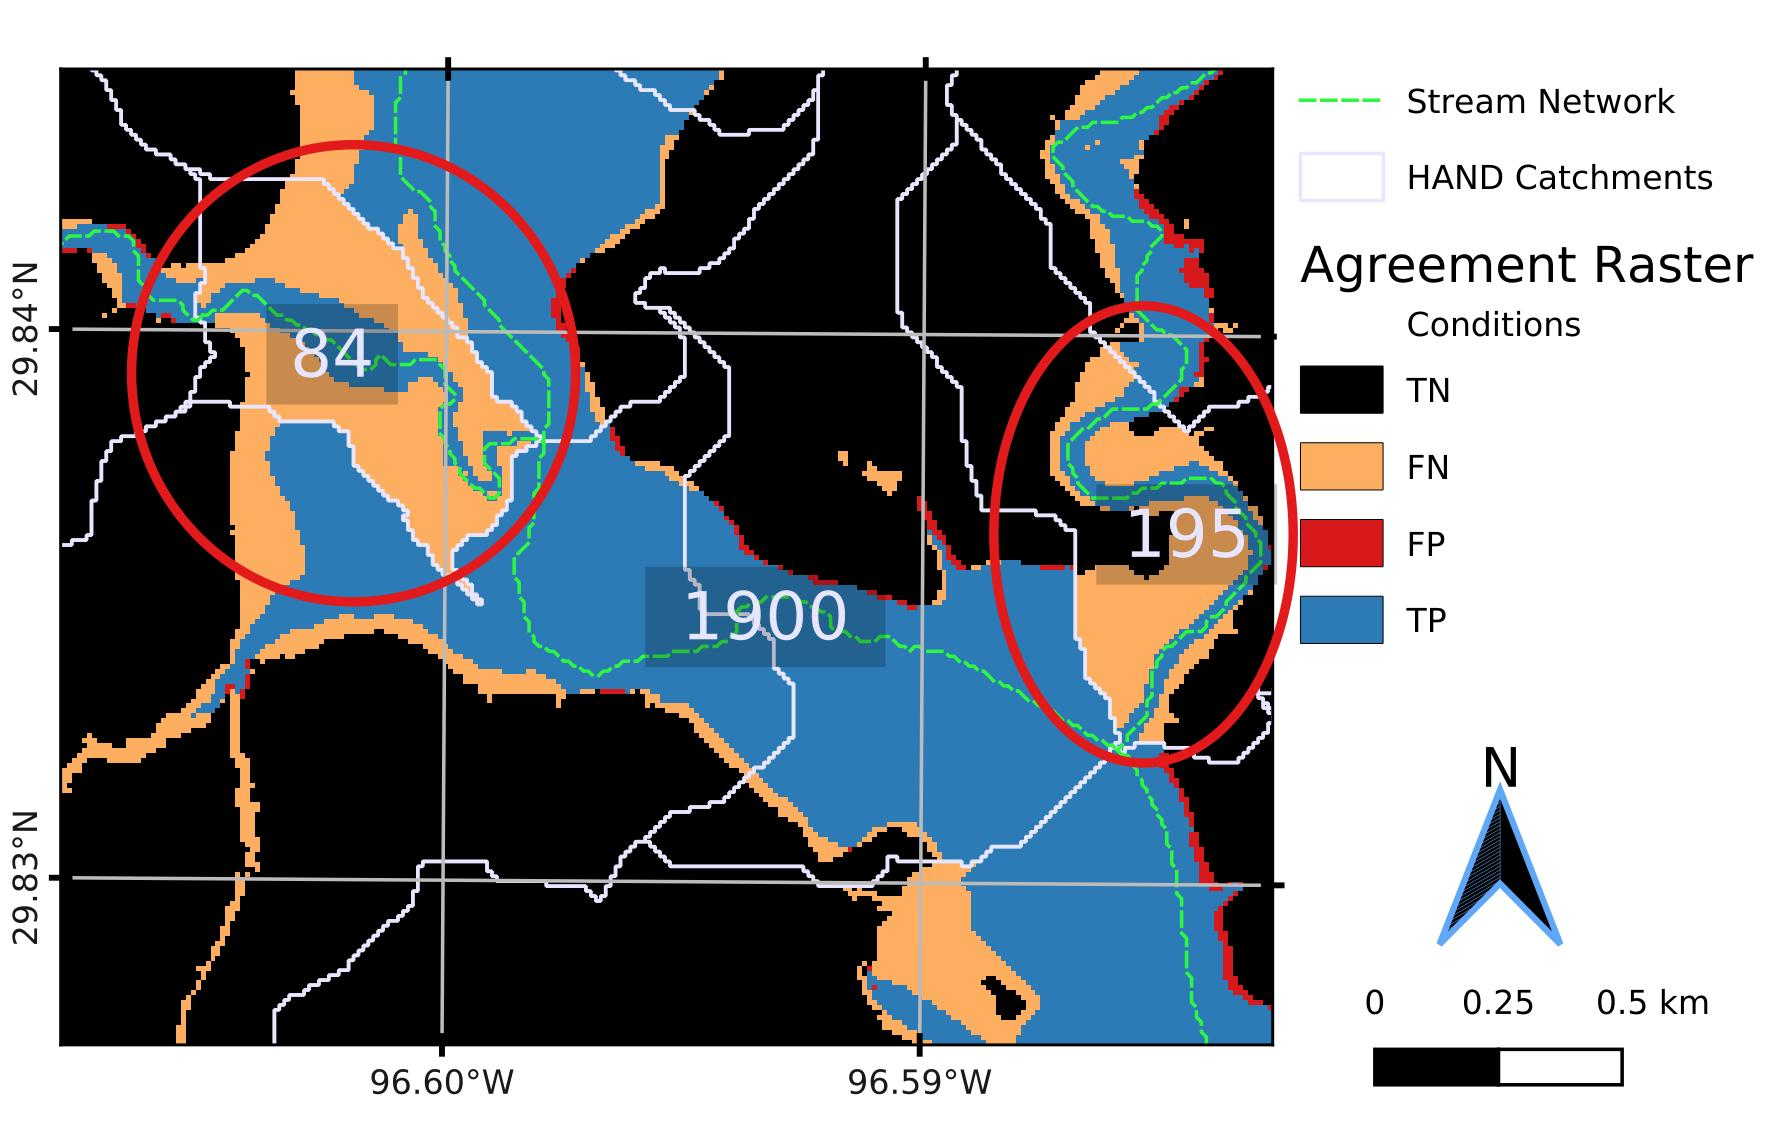
\includegraphics[scale=1.0]{figures/catchment_boundaries_issue.jpg}
\caption{False negatives associated with confluence of tributaries with mainstems. Integers represent flow values from BLE 100 year for the associated areas. No backwater consideration is implemented and the independent nature of the HAND catchments prohibits pluvial inundation from taking place.}
\label{fig:catchment_boundaries_issue}
\end{figure}
%
The limitation imposed by using stream networks of Horton-Strahler stream order \cite{horton1945erosional,strahler1952hypsometric,strahler1952hypsometric} greater than one for HAND can be described mathematically with Graph Theory.
Assume a drainage area denoted by special case of a fully connected, directed acyclic graph known as a tree, G, with all nodes (or reaches) directed from the leaf nodes (or headwater reaches) toward a singular root node $r_0$ known as the outlet in the application's field.
Assume a singluar subgraph of G where by a new root node, $r_n$, is introduced that represents another stream location.
n is used here to index possible root nodes which are a subset of G.
Ensuring $r_n$ is itself an inner node (has upstream drainage) disconnects G into $G_0$ and $G_n$ thus removing influence of conditions at $r_0$ upon $G_n$.
HAND seeks to divide drainage areas into reach scale catchments that are independent of one another.
We intend to demonstrate how introduction of stream orders greater than one can generate errors at confluences.
We present two successive methods implemented that reduce drainage densities by reducing Horton-Strahler stream orders of the networks employed and test our presented hypothesis that unary stream order networks enhance FIM performance skill with HAND.
%
%%%%%%%%%%%%%%%%%%%%%%%%%%%%%%%%%%%%%%%%%%%%%%%%%%%%%%%%
\subsubsection{NWS Replace and Route Mainstems}
\label{sssec:replace_and_route_mainstems}
%
The RnR configuration of the NWM seeks to replace NWM forecasts by assimilating best available AHPS forecasts and routing them downstream.
The RnR Mainstems (MS) network is a subset of the NWM full-resolution (FR) network at and downstream of AHPS forecast points.
The RnR MS network, or simply MS, comprises about 200 thousand km of stream length which is less than 4\% of the FR total stream length of 5.5 million km.
HAND was originally derived for this stream network to enhance mapping skill along these critical MS \cite{djokic2019arc}. 
The inundation derived from this stream network is mosaiced or composited with the inundation from the FR network to form composite (C) FIMs. 
Within each HAND processing unit (HUC 4, 6, 8), you'll typically only find a MS stream network of stream order 1.
%
%%%%%%%%%%%%%%%%%%%%%%%%%%%%%%%%%%%%%%%%%%%%%%%%%%%%%%%%
\subsubsection{Generalized Mainstems}
\label{sssec:generalized_mainstems}
%
To further the efforts implmented by MS, we sought to derive HAND at a level-path scale which we call Generalized Mainstems (GMS).
Level-path groups flow paths by maximizing the length of each flow path and minimizing the number of level path identifiers within a given domain. 
Starting at the outlet, a unique level-path is propogated upstream. 
At every confluence, the direction of maximum flow path length is sought to propogate the current level-path identifier.
For the remaining parent reaches of the given junction, a new level-path identifier is assigned and the process recursively continues with them.
Each HUC 4,6,or 8 is discretized into level-paths indepedently and relevant inputs are assigned to each level-path processing unit given a buffer of 7 km.
At the level-path scale, the methods in Section \ref{ssec:deriving_fim_hydrofabric} are executed while the methods in Section \ref{ssec:hydro_conditioning} are still completed at the HUC scale.
%
%%%%%%%%%%%%%%%%%%%%%%%%%%%%%%%%%%%%%%%%%%%%%%%%%%%%%%%%
\subsection{Inundation Mapping}
\label{ssec:inundation_mapping}
%
The FIM hydrofabric consisting of the relative elevations grid, catchments grid, catchment polygons, rating curve, and cross-walking data are all used to convert forecasts from the NWM into forecasts extents.
For operational situations, one would cache the FIM hydrofabric then either produce libraries of FIM for a sample of discharges or stages or also produce the FIM in near real-time (NRT).
From the cached FIM hydrofabric and design or forecast discharges including those extracted from the NWM, inundation maps can be generated at HUC 4, 6, or 8 spatial processing units in a rapid, parallel operation. 
The discharges are associated with NWM reach identifiers and cross-walked over to reach identifiers in the FIM hydrofabric.
Once associated to a mapping stream network, the catchments grid encoded with the reach identifiers are used to map the stages by thresholding to the forecast stage.
Mathematically, the catchment pixels, $C_{ij}$, can be indexed by the reach identifiers, i, and pixel indices, j.
For each forcast stage, $S_i$, one can express the formula for $F_{ij}$, a binary variable denoting inundation condition in equation \ref{eq:hand_fim}.
%
\begin{equation}
\label{eq:hand_fim}
    F_{ij} = 
    \begin{cases}
        1 & if S_i > C_{ij} \\
        0 & else
    \end{cases}
\end{equation}
%
For the cases of MS and GMS, the inundations must be mosaiced together to form a seamless forecast.
For MS, the inundation from MS stream network is unioned with the FR inundation extents while all the individual level-path inundation extents are unioned to form the composite inundation, C, for GMS.
Equation \ref{eq:comp_fim} illustrates how the composite inundation, C, can be determined from n sources,F, all indexed by i.
%
\begin{equation}
\label{eq:comp_fim}
    C = \cup_{i=1}^{n}F_i
\end{equation}
In the case of MS, the n value is 2 for the FR and MS inundation sources while for GMS n is equivalent to the number of unique level-paths in the domain of concern.
%
%%%%%%%%%%%%%%%%%%%%%%%%%%%%%%%%%%%%%%%%%%%%%%%%%%%%%%%%
\subsection{Evaluation and Calibration}
\label{ssec:evaluation_and_calibration}
%%%%%%%%%%%%%%%%%%%%%%%%%%%%%%%%%%%%%%%%%%%%%%%%%%%%%%%%
%
Evaluation of the OWP-FIM V3 Cahaba is conducted by comparison to the HEC-RAS 1D derived models produced by FEMA region 6 \cite{fema2021base,fema2021estimated}.
The maps to the 1\% recurrence flow (1 in 100 year) and the 0.2\% recurrence flow (1 in 500 year) are furnished by FEMA so we used those corresponding discharges and mapping extents for evaluation.
By not using the same HEC-RAS derived discharges and FIM extents, we are able to separate out errors imputed by hydrology, forcings, hydraulic routing, etc that we would have potentially seen if we used NWM forecasted discharges.
We elected to spatially intersect the HEC-RAS cross sections with the NWM stream network assigning the 1\% and 0.2\% flow rates with each NWM reach. 
To handle multiple intersections, we opted to use a filter to select the median discharge value attributed to each NWM reach.
This partially handles the influence of neighboring cross sections that could cause flow discontinuties and mass conservation issues.
Additionally, the stream network of the FEMA furnished models are of higher stream densities and bifurcation ratios leading to a signicant amount of false negatives (FN) (under-prediction) along headwater streams with Horton-Strahler orders of one due to the lack of representation of these additional headwater streams in the NWM network.
While the limitions are noted, this method does best detangle the influence of exogeneous variables that we do not wish to study in this comparison.

The metrics employed in this study to evaluate inundation extents include critical success index (CSI), probability of detection (POD), and false alarm ratio (FAR) and presented in equations \ref{eq:csi}, \ref{eq:pod}, \ref{eq:far}, respectively.
To calculate these secondary metrics, one must define three primary metrics including true positives (TP) which is predicted wet and wet in benchmark dataset.
The two types of errors consist of false positives (FP), or type I errors, which is dry in benchmark but predicted wet and false negatives (FN), or type II errors, which is wet in benchmark by predicted dry. 
Lastly, the reader may come across true negatives (TN) which is defined as dry in both the benchmark and predicted datasets.
Maximizing POD indicates a model's ability to detect the given threat of interest, inundation, while minimizing FAR is sought to indicate a models ability in reducing FN errors.
The NWS denotes CSI a good proxy for measuring a forecasting systems utility in protecting life and property and has been shown to be optimized mathematically when $POD = 1 - FAR$ \cite{gerapetritis2004behavior}.
While these metrics are commonly employed in the evaluation of FIM and binary weather prediction communities in general, they do come with some notable limitations including frequency dependence in the case of CSI and FAR \cite{gerapetritis2004behavior,stephens2014problems,schaefer1990critical,jolliffe2012forecast}.
Thus frequency dependent statistics should be used with caution. 
%
\begin{equation}
\label{eq:csi}
CSI = \frac{TP}{TP + FN + FP}
\end{equation}
%
\begin{equation}
\label{eq:pod}
POD = \frac{TP}{TP + FN}
\end{equation}
%
\begin{equation}
\label{eq:far}
FAR = \frac{FP}{TP + FP}
\end{equation}
%
Calibrating the Manning's n values is very important for optimizing the skill of inundation extent forecasts \cite{zheng2018river,garousi2019terrain}.
\note[Fernando Aristizabal]{For Brian Avant} In this study we propose a simplified parameterization of roughness by stream order and tune inundation performance relative to the validation data set.
For every combination of stream order (from 1 to 14) and Manning's n value (from X.XX to X.XX), synthetic rating curves are generated and compared to the FEMA inundation extents.
The optimal roughness for each stream order is determined by maximizing CSI.
A clear limitation of this approach is over-fitting to the BLE domain at 1\% and 0.2\% recurrence discharges.
On-going work is focused on applying more advanced techniques through use of USGS stream gage rating curves.
%
